%!TeX root=Final.tex

\chapter{PRODUCT SPACES}\label{chapter:product spaces}

Often times in topology or algebra, when working with a structure (be it a topological space, a group, a ring...) it is interesting or convenient to be able to create \emph{product} structures; that is, equip a cartesian product with the same structure their components had\footnote{The categorical process that justifies this is the \emph{product universal property}.}. In this chapter, we aim to construct said product in measure spaces.

It is convenient to warn the reader that the notation used in this chapter 
is, to the writer's knowledge, original, and in any case different to that found in \cite{ash1972real}.
\section{Finite product of measure spaces}\label{subsection:product measures}

We will begin our study of product measure spaces with the finite case. As we will see, the \emph{algebraic} part of this - the part regarding measurability and \(\sigma\)-fields - is rather easy and done very similarly to how it is done in topology. In the \emph{analytical} details - that is, when measures take play - is where most of the theory arises.

We will develop first the \emph{algebraic} part: the structures where we will work. As in topology, it is desirable that cartesian products of sets in the base structures also belong to the product structure. 

\begin{defn}
  Let \(\mathcal{F}_{j}\) be a \(\sigma\)-field of subsets of some set \(\Omega_{j}, j=1,\dotsc,n\). Define \(\Omega=\Omega_{1}\times\dotsc\times\Omega_{n}\). A \textbf{measurable rectangle} of \(\mathcal{F}_{1},\dotsc,\mathcal{F}_{n}\), or, for short, a \textbf{rectangle} in \(\Omega\) is a set \(A\subseteq\Omega\) of the form \(A=A_{1}\times\dotsc\times A_{n}\), with \(A_{i}\in\mathcal{F}_{i}\).

  The smallest \(\sigma\)-field over \(\Omega\) containing all measurable rectangles of \(\mathcal{F}_{1},\dotsc,\mathcal{F}_{n}\) is called the \textbf{product} \(\pmb{\sigma}\)\textbf{-field}, and is denoted by \(\mathcal{F}_{1}\times\dotsc\times\mathcal{F}_{n}\) (this is not the cartesian product of the sets \(\mathcal{F}_{1},\dots,\mathcal{F}_{n}\)). If \(\mathcal{F}_1=\dotsc=\mathcal{F}_n=\mathcal{F}\) for some \(\sigma\)-field \(\mathcal{F}\), we denote \(\mathcal{F}^n=\mathcal{F}_1\times\dots\times\mathcal{F}_n\).

  Consider a finite, proper subset \(v\subseteq \{1,\dots,n\}\). Write \(v= \{i_1,\dots,i_r\}\), and
  \(v^c=\{j_1,\dots,j_l\}\) (then, \(n=r+l\)), with \(i_1<\dots<i_r\) and \(j_1<\dots<j_l\). Fix the values
  \(\omega_{i_1},\dots,\omega_{i_r}\), with \(\omega_{i_k}\in\Omega_{i_k}\).
  Define the \textbf{section} of a given set \(F\subseteq\Omega\) at \(\omega_{i_1},\dots,\omega_{i_r}\) as
  \[F^{\omega_{i_1},\dots,\omega_{i_r}}=\left\{\left(\omega_{j_1},\dots,\omega_{j_l}\right)\in\Omega_{j_1}\times \dots\times \Omega_{j_l}\left|\left(\omega_1,\dotsc,\omega_n\right)\in F\right.\right\}.\]
  Finally, define the \textbf{section} of a given function \(f\colon \Omega\to X \) (where \(X\) is some arbitrary set) at \(\omega_{i_{1}}, \dots , \omega_{i_{r}}\) as the function \(f^{\omega_{i_{1}}, \dots , \omega_{i_{r}}}\colon\Omega_{j_{1}}\times \dots \times \Omega_{j_{l}}\to X\) Such that \((\omega_{j_{1}}, \dots , \omega_{j_{l}})\mapsto f(\omega_1,\dots,\omega_n)\).
\end{defn}

\begin{figure}[!h]
    \centering
    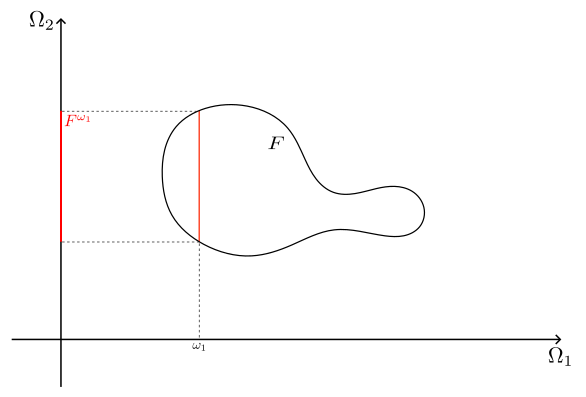
\includegraphics[width=0.9\linewidth]{resources/figures/section.png}
    \caption{Section \(F^{\omega_1}\) of a subset \(F\) of a product of two measurable spaces, \(\Omega_1\) and \(\Omega_2\).}
    \label{figure:section}
\end{figure}

Sections have very interesting properties regarding set operations and measurable spaces.

\begin{prop}[Properties of sections]\label{proposition:properties of sections}Under the notation of the previous definition, let \(\{A_t\left|t\in T\right.\}\) be an arbitrarily indexed collection of subsets of ~\(\Omega=\Omega_1\times\dots\times\Omega_n\).\footnote{This result is original.} Then,

\begin{enumerate}
    \item\label{proposition:properties of sections 1} For every fixed values \(\omega_{i_1},\dots,\omega_{i_r}\), with \(\omega_{i_k}\in\Omega_{i_k}\), one has
    \[
        \left(\bigcup_{t\in T}A_t\right)^{\omega_{i_1},\dots,\omega_{i_r}}= \bigcup_{t\in T} A_t^{\omega_{i_1},\dots,\omega_{i_r}} \text{ ~and~ }
        \left(\bigcap_{t\in T}A_t\right)^{\omega_{i_1},\dots,\omega_{i_r}}= \bigcap_{t\in T} A_t^{\omega_{i_1},\dots,\omega_{i_r}} 
    .\]
    Additionally, for every set \(A\in\Omega\),
        \[\left(A^{\omega_{i_1},\dots,\omega_{i_r}}\right)^{c}=\left(A^c\right)^{\omega_{i_1},\dots,\omega_{i_r}}.\]

    \item\label{proposition:properties of sections 2} For every fixed values \(\omega_{i_1},\dots,\omega_{i_r}\), with \(\omega_{i_k}\in\Omega_{i_k}\), \(\emptyset^{\omega_{i_1},\dots,\omega_{i_r}}=\emptyset\). In particular, if the sets \(A_t\) are disjoint pairwise, so are the sections 
    \(A_t^{\omega_{i_1},\dots,\omega_{i_r}}\).
    \item\label{proposition:properties of sections 3} Sections of measurable sets are always measurable in their respective \(\sigma\)-fields.
		\item\label{proposition:properties of sections 4} Sections of measurable functions are always measurable in their respective \(\sigma\)-fields.
\end{enumerate}
\end{prop}
\begin{proof}
\begin{enumerate}
    \item This proof is a simple verification of quantifiers. We will omit it.
    \item Clearly, a section of the empty set is empty. Moreover, if \(A\) and \(B\) are disjoint subsets of \(\Omega\), then, by 
        \ref{proposition:properties of sections 1}, \[A^{\omega_{i_1},\dots,\omega_{i_r}}\cap B^{\omega_{i_1},\dots,\omega_{i_r}}=(A\cap B)^{\omega_{i_1},\dots,\omega_{i_r}}=\emptyset^{\omega_{i_1},\dots,\omega_{i_r}}=\emptyset.\]
    \item Write \(\mathcal{F}=\mathcal{F}_1\times\dotsc\times\mathcal{F}_n\),
  %\(\Omega_{v^c}=\Omega_{j_1}\times\dotsc\times\Omega_{j_l}\)
  and \(\mathcal{F}_{v}=\mathcal{F}_{j_1}\times \dotsc\times\mathcal{F}_{j_l}\).

  Define the class of sets \(\mathcal{C}=\{B\in\mathcal{F}|F^{w_{i_1},\dotsc,w_{i_r}}\in\mathcal{F}_v\}\).
  It is clear that \(\mathcal{C}\) is a \(\sigma\)-field, because of \ref{proposition:properties of sections 1} and the fact that \(\mathcal{F}_{v}\) is a \(\sigma\)-field. Additionally, \(\mathcal{C}\) contains all measurable rectangles, because
  \[(A_{1}\times\dotsc\times A_n)^{w_{i_1},\dotsc,w_{i_r}}=\left\{
          \begin{array}{rl}
              A_{j_1}\times\dotsc\times A_{j_l}, & \text{ if } (w_{i_1},\dotsc,w_{i_r})\in A_{i_1}\times\dotsc\times A_{i_r},\\
              \emptyset, & \text{ otherwise.}
      \end{array}\right.\]
Thus, \(\mathcal{F}=\mathcal{C}\).
\item This is an immediate consequence of \ref{proposition:properties of sections 3} and the fact that, for any given set \(Z\subseteq X\),
    \[
        \left(
        f^{\omega_{i_{1}}, \dots , \omega_{i_{r}}}
        \right)^{-1}(Z)=\left(f^{-1}(Z)\right)^{\omega_{i_{1}}, \dots , \omega_{i_{r}}}
    .\]
\end{enumerate}
\end{proof}
\begin{remk}
In a given product measurable space, the class of disjoint unions of measurable rectangles forms a field.
\end{remk}

We have now covered the \emph{algebraic} part of the section. We have developed the structure on which we will measure, and now wish to construct measures on these product spaces using measures on the base spaces.

The following theorem does this for the \(n=2\) case. The intuition behind it can be explained in terms of \Cref{figure:section}. If we want to measure a set \(F\subseteq\Omega_1\times\Omega_2\) we can consider, for every \(\omega_1\in\Omega_1\), the intersection between the vertical line at \(\omega_1\) and the set \(F\). This intersection is parallel to the section \(F^{\omega_1}\), which we are able to measure since it is a measurable subset of \(\Omega_2\). The way we measure \(F^{\omega_1}\) can be the same for each \(\omega_1\)\footnote{This is the approach followed in the ``classical'' Product Measure Theorem; see \Cref{corollary:classical Product Measure}.}, or can vary depending on it, so that we have a different measure \(\mu^{\omega_1}\) on \(\Omega_2\) for every \(\omega_1\). Finally, to measure \(F\) we can integrate all of the different values obtained for each \(\omega_1\) with respect to a given measure on \(\Omega_1\). Finally, we need to impose some technical constraints regarding measurability and \(\sigma\)-finiteness, which are included in the statement of the result.

\begin{thrm}[Two-Dimensional Product Measure Theorem]\label{theorem:two-dim Product Measure}
  Let \(\left(\Omega_{1},\mathcal{F}_{1}\right)\) and \linebreak \(\left(\Omega_2,\mathcal{F}_2\right)\) be measurable spaces, and \(\mu\) a \(\sigma\)-finite measure on \(\mathcal{F}_{1}\). Assume that we are given a map
  \(\mu\colon\Omega_{1}\times\mathcal{F}_{2}\to \overline{\mathbb{R}}\) which satisfies:
  \begin{itemize}
	\item The mapping \(\mu^{\omega_1}=\mu(\omega_{1},\cdot)\) is a measure over \(\mathcal{F}_{2}\) for every fixed \(\omega_{1}\in\Omega_{1}\).
	\item \(\mu(\cdot,B)\) is \(\mathcal{F}_{1}\)-measurable for every fixed \(B\in\mathcal{F}_{2}\). \footnote{Here it is convenient to remind the reader that, unless explicitly stated otherwise, the reals and extended reals are always equipped with the Borel \(\sigma\)-field.}
	\item \(\mu\) is uniformly \(\sigma\)-finite; that is, \(\Omega_{2}\) can be written as \(\bigcup_{n}B_{n}\), where \(B_n\in\mathcal{F}_2\) and there exist some constants \(k_{n}\in\mathbb{R}^{+}\) such that \(\mu(\omega_{1},B_{n})\leq k_{n}\) for all \(\omega_{1}\in\Omega_{1}\). %and all \(n\in\mathbb{N}\).
  \end{itemize}

  Then, there is a unique measure \(\mu\) on \(\mathcal{F}=\mathcal{F}_{1}\times\mathcal{F}_{2}\) such that
  \[\mu(A\times B)=\int_A \mu^{\omega_1}(B)~d\mu_1 \text{ for every measurable rectangle } A\times B.\]
  Namely,
  \[\mu(C)=\int_{\Omega_1}\mu^{\omega_1}(C^{\omega_1})~d\mu_1.\]
  Furthermore, \(\mu\) is \(\sigma\)-finite on \(\mathcal{F}\); and if \(\mu_1\) and all the \(\mu^{\omega_1}\) are probability measures, so is \(\mu\).
\end{thrm}
\begin{proof}
Define the function \(s(\omega_1,F)=\mu\left(\omega_1,F^{\omega_1}\right)\).

  \begin{enumerate}
      \item[1.] First assume that the \(\mu^{\omega_1}\) are finite.
          We will start by showing that the function
		  \(s(\cdot,F)\) is measurable for every \(C\in\mathcal{F}\).

		  Let \(\mathcal{C}\) be the class of sets of \(\mathcal{F}\) for which the function is measurable.
		  Note that \(\mathcal{C}\) contains all measurable rectangles: take \(C=A\times B\).
		  Then,
		  \[\mu^{\omega_1}(F^{\omega_1})=\mu(\omega_{1	},F^{\omega_1})=\left\{\begin{array}{rl}
													 \mu(\omega_{1	},A),& \text{ if }\omega_{1	}\in A,\\
													 0,& \text{ otherwise.}

												   \end{array}\right.\]
Thus, \(\mu^{\omega_1}(F^{\omega_1})=\mu^{\omega_1}(A)I_A(\omega_1)\),
          which is clearly measurable.

					We will now use the \hyperref[theorem:Monotone Class]{Monotone Class Theorem}
          to show that \(s(\cdot,F)\) is measurable for all \(F\in\mathcal{F}\). Let \(\mathcal{F}_0\) be the
          field of disjoint unions of measurable rectangles.

          It is clear that \(\mathcal{F}_0\subseteq\mathcal{C}\), since, if
          \(C_1,\dotsc,C_n\) are disjoint measurable rectangles in  \(\mathcal{F}\), then for any
          given \(\omega_1\in\Omega_1\), from \Cref{proposition:properties of sections 1} and \Cref{proposition:properties of sections 2} 
          it is deduced that \(\mu^{\omega_1}(\left(
          \bigcup_{k}C_k\right)^{\omega_1})=\sum_{k}\mu^{\omega_1}\left(C_k^{\omega_1}\right)\),
          which is a finite sum of Borel measurable functions; thus measurable.

          If we now show that \(\mathcal{C}\) is a monotone class, it will follow
          that \(\mathcal{F}=\sigma\left(\mathcal{F}_0\right)=\mathcal{C}\). If 
          \(A_n\uparrow A\), then  \(A_n^{\omega_1}\uparrow 
          A^{\omega_1}\). By \Cref{proposition:limit of increasing sets}, 
          we have \(\mu^{\omega_1}\left( 
          A_n^{\omega_1}\right)\to\mu^{\omega_1}\left(A^{\omega_1}\right)\); that is, \(s(\omega_1,A_n^{\omega_1})\to s(\omega_1,A^{\omega_1})\). Since a pointwise limit of measurable functions is measurable, we have  \(A^{\omega_1}\in\mathcal{C}\).
          Similarly, from the fact that all the measures are finite and \ref{proposition:limit of decreasing sets}, it
          follows that \(\mathcal{C}\) also contains all descending limits
          of sets in it. Thus, \(\mathcal{C}=\mathcal{F}\). This guarantees
          that \(\mu\) is well-defined.

          Now it is easy to see that \(\mu\) is a measure. Nonnegativity is immediate. Following \Cref{corollary:exchange series and integral}, and \Cref{proposition:properties of sections 2},
          \[
              \begin{aligned}
                  \mu\left(\bigcup_{n}A_n\right)=&     
                  \int_{\Omega_1}\mu^{\omega_1}\left(\left(\bigcup_{n}A_n\right)^{\omega_1}\right)~d\mu_1 \\
                  =& \int_{\Omega_1}\sum_{n} \mu^{\omega_1}\left(A_n^{\omega_1}\right)~d\mu_1\\
                  =& \sum_{n} \int_{\Omega_1}\mu^{\omega_1}(A_n^{\omega_1})~d\mu_1 \\
                  =& \sum_{n} \mu(A_n).
              \end{aligned}
          \]

      Finally, note that \[ \mu(A\times
          B)=\int_{\Omega_1}\mu^{\omega_1}(\left(A\times  B\right)^{\omega_1})~d\mu_1=\int_{\Omega_1}I_A(\omega_1)\mu^{\omega_1}(B)~d\mu_1=\int_{A}\mu^{\omega_1}(B)~d\mu_1.
      \]
      
  \item[2.] Now assume the \(\mu^{\omega_1}\) to be uniformly \(\sigma\)-finite. Note that the sets \(B_n\) may be assumed to be disjoint without loss of generality: simply take \(B_n'=B_n\setminus \bigcup_{k=1}^{n-1}B_k\). Then, \(\mu(\omega_1,B_n')\leq\mu(\omega_1,B_n)\leq k_n\) for every \(\omega_1\).

Define \(\mu_n(\omega_1,B)=\mu(\omega_1,B\cap B_n)\) for each \(n\). 
Note that \(\mu^{\omega_1}=\sum_{n} \mu_n^{\omega_1}\) for every \(\omega_1\) (where \(\mu_n^{\omega_1}=\mu_n(\omega_1,\cdot)\). Apply the construction above to each \(\mu_n\). Then,
define a measure on \(\mathcal{F}\) by
\[
\mu(C)=\sum_{n} \mu_n(C)
.\] 
This measure will satisfy
\[
    \mu(C)=\sum_{n}\int_{\Omega_1}\mu_n^{\omega_1}(C^{\omega_1})~d\mu_1
    =\int_{\Omega_1}\sum_{n}\mu_n^{\omega_1}(C^{\omega_1})~d\mu_1
    =\int_{\Omega_1}\mu^{\omega_1}(C^{\omega_1})~d\mu_1
,\]
which implies, again, that for measurable rectangles \(\mu(A\times B)=\int_{A}\mu^{\omega_1}(B)~d\mu_1\).
\end{enumerate}

For the uniqueness part of the result, we will employ the \hyperref[theorem:Caratheodory Extension]{Carathéodory Extension Theorem}, by showing that \(\mu\) is \(\sigma\)-finite on \(\mathcal{F}_0\), the field of disjoint unions of measurable rectangles.

Since \(\mu_1\) is \(\sigma\)-finite, we can find a sequence of sets \(A_1,A_2,\dots\) such that \(\mu_1(A_m)<\infty\) and \(\Omega_1=\bigcup_{m}A_m\). Define \(C_{nm}=A_m\times B_n\), so that \(\Omega=\bigcup_{nm}C_{nm}\). Additionally,

\[\mu(C_{nm})=\int_{A_m}\mu^{\omega_1}(B_n)~d\mu_1\leq k_n\mu_1(A_m)<\infty.\] 
We have just seen that \(\mu\) is \(\sigma\)-finite on \(\mathcal{F}_0\subseteq\mathcal{F}\), hence on \(\mathcal{F}\). If \(\mu_1\) and all functions \(\mu^{\omega_1}\) are probability measures, it is immediate that \(\mu\) is so too.
\end{proof}
A very natural question to ask now is how does integration with respect to this new measure relates with integration with respect to the ``original'' measures \(\mu_1\) and \(\mu^{\omega_1}\). The following theorem answers with detail this question.

\begin{thrm}[Two-Dimensional Fubini's Theorem]\label{theorem:two-dim Fubini's}
    Under the hypotheses and notation of \Cref{theorem:two-dim Product Measure}, let \(\Omega=\Omega_1\times\Omega_2\), and \(f\colon \Omega\to\overline{\mathbb{R}}\) be a \(\mathcal{F}\)-measurable function. For every fixed \(\omega_1\in\Omega_1\), consider the section \(f^{\omega_1}\colon\Omega_2\to\overline{\mathbb{R}}\). Then,
    \begin{enumerate}
        \item If \(f\) is nonnegative, then the function \(F(\omega_1)=\int_{\Omega_2}f^{\omega_1}d\mu^{\omega_1}\) exists and is \(\mathcal{F}_1\)-measurable. Also,
            \begin{equation}\label{equation:two-dim Fubini's}
                \int_{\Omega}f~d\mu=\int_{\Omega_1}F~d\mu_1=\int_{\Omega_1}\left(\int_{\Omega_2}f^{\omega_1}~d\mu^{\omega_1}\right)~d\mu_1
            \end{equation}
        \item If \(\int_{\Omega}f~d\mu\) exists (respectively, is finite), then \Cref{equation:two-dim Fubini's} holds in the sense that the function \(F(\omega_1)=\int_{\Omega_2}f^{\omega_1}~d\mu^{\omega_1}\) exists (respectively, is finite) for \(\mu_1\)-almost every \(\omega_1\), and defines a Borel measurable function of \(\omega_1\) if it is taken as \(0\) on the exceptional set (or as any Borel measurable function).
    \end{enumerate}
\end{thrm}
\begin{proof}
    \begin{enumerate}
        \item \(F\) exists because \(f^{\omega_1}\) is nonnegative for every \(\omega_1\). Start by suppossing that \(f\) is an indicator, \(I_C\). Then, it is not hard to see that \(f^{\omega_1}=I_{C^{\omega_1}}\). Thus,
        \[
            F(\omega_1)=\int_{\Omega_2}I_{C^{\omega_1}}~d\mu^{\omega_1}=\int_{C^{\omega_1}}~d\mu^{\omega_1}=\mu^{\omega_1}(C^{\omega_1})
        ,\]
        which is \(\mathcal{F}_1\)-measurable, as we saw in the proof of \Cref{theorem:two-dim Product Measure}. Additionally, \(\int_{\Omega}f~d\mu=\mu(C)=\int_{\Omega_1}\mu^{\omega_1}(C^{\omega_1})~d\mu_1=\int_{\Omega_1}F(\omega_1)~d\mu_1\), by that same theorem.

        Now suppose \(f\) is a simple, nonnegative function \(\sum_{i} x_iI_{C_i}\). Then, by linearity, \(F(\omega_1)=\sum_{i} x_i\mu^{\omega_1}(C_i^{\omega_1})\), which is a measurable function and satisfies that
        \[
            \int_{\Omega}f~d\mu=\sum_{i} x_i\int_{\Omega}I_{C_i}~d\mu=\int_{\Omega_1}F~d\mu_1
        .\]
				For an arbitrary nonnegative, Borel measurable function \(f\), consider a sequence of nonnegative, simple functions \(s_n\uparrow f\). Define \(F_n(\omega_1)=\int_{\Omega_2}s_n^{\omega_1}~d\mu^{\omega_1}\). By what we have seen for simple functions, \(F_n\) is measurable. By the \hyperref[theorem:Monotone Convergence]{Monotone Convergence Theorem}, \(F_n\uparrow F\) pointwise, and thus \(F\) is measurable.
        Applying the \hyperref[theorem:Monotone Convergence]{Monotone Convergence Theorem} again, this time twice, it follows that
        \[
            \int_{\Omega_1}F~d\mu_1=\lim_n\int_{\Omega_1}F_n~d\mu_1=\lim_n\int_{\Omega}s_n~d\mu=\int_{\Omega}f~d\mu
        .\]
    \item Split \(f=f^{+}-f^{-}\). Note that \((f^{\omega_1})^{+}=\left(f^{+}\right)^{\omega_1}\), and \((f^{\omega_1})^{-}=\left(f^{-}\right)^{\omega_1}\). Apply the construction above to \(f^{+},f^{-}\), and obtain two functions \(F^{+}, F^{-}\). Note that \(F(\omega_1)\) exists if, and only if, at least one of \(F^{+}(\omega_1),F^{-}(\omega_1)\) is finite, and in that case \(F(\omega_1)=F^{+}(\omega_1)-F^{-}(\omega_1)\).

    Since \(\int_{\Omega}f~d\mu\) exists, at least one of \(f^{+},f^{-}\) is integrable. Suppose, without loss of generality, that \(\int_{\Omega}f^{+}~d\mu<\infty\). Then,
    \[
        \int_{\Omega_1}F^{+}~d\mu_1=\int_{\Omega}f~d\mu<\infty
    ,\]
    by the first section of this theorem. Hence, \(F^{+}\) is finite \(\mu_1\)-a.e., and \(F=F^{+}-F^{-}\) exists whenever this is the case, and is measurable if taken as \(0\) (or any measurable function) elsewhere. Finally,
    \[
        \int_{\Omega}f~d\mu=\int_{\Omega}f^{+}~d\mu-\int_{\Omega}f^{-}~d\mu=\int_{\Omega_1}F^{+}~d\mu_1-\int_{\Omega_2}F^{-}~d\mu_1=\int_{\Omega_1}F~d\mu_1
    .\]
    \end{enumerate}
The third integral is simply a different notation for the second integral.
\end{proof}
\begin{remk}\label{remark:two-dim Fubini's on subsets}
    In the last theorem, if we wish to integrate \(f\) in some measurable subset \(C\) of ~\(\Omega\), simply consider \(g=I_Cf\), which is measurable. Then, \(\int_{\Omega}g~d\mu\) exists if \(\int_{\Omega}f~d\mu\) does and \(g^{\omega_1}=I_{C^{\omega_1}}f^{\omega_1}\). Thus,
    \[
        \int_{C}f~d\mu=\int_{\Omega}g~d\mu_1=\int_{\Omega_2}\int_{C^{\omega_1}}f^{\omega_1}~d\mu^{\omega_1}~d\mu_1
    .\]
\end{remk}
Having covered the \(n=2\) case, we can now inductively extend the last two theorems to products of \(n\) measurable spaces.

\begin{thrm}
    Let \(\left(\Omega_j,\mathcal{F}_j\right)\) be measurable spaces, \(j=1,\dots,n\), and \(\mu_1\) a \(\sigma\)-finite measure on \(\mathcal{F}_1\). Assume that, for each \(j=1,\dots,n-1\), we are given a map \(\mu_{j+1}\colon\Omega_1\times\dots\times\Omega_j\times\mathcal{F}_{j+1}\to\overline{\mathbb{R}}\) that satisfies
\begin{itemize}
    \item The mapping \(\mu^{\omega_1,\dots,\omega_j}=\mu_{j+1}(\omega_1,\dots,\omega_j,\cdot)\) is a measure over \(\mathcal{F}_{j+1}\) for every fixed \(\omega_1\in\Omega_1,\dots,\omega_j\in\Omega_j\).
    \item \(\mu_{j+1}(\cdot,\dots,\cdot,B)\) is \( \left(\mathcal{F}_1\times\dots\times\mathcal{F}_j\right)\)-measurable for every fixed \(B\in\mathcal{F}_{j+1}\).
    \item \(\mu_{j+1}\) is uniformly \(\sigma\)-finite, that is, \(\Omega_{j+1}\) can be written as \(\bigcup_{r}B_{(j+1)r}\), where \(B_{(j+1)r}\in\mathcal{F}_{j+1}\) and there exist some constants \(k_n\in\mathbb{R}^{+}\) such that \(\mu_{j+1}(\omega_1,\dots,\omega_j,B_n)\leq k_n\) for all \(\omega_1\in\Omega_1,\dots,\omega_j\in\Omega_j\).
\end{itemize}
Then,

\begin{enumerate}
    \item \emph{\textbf{Product Measure Theorem.}} \label{theorem:Product Measure} There exists a unique measure \(\mu\) on \(\mathcal{F}=\mathcal{F}_1\times\dots\times\mathcal{F}_n\) such that
\[
    \mu(A_1\times\dots\times A_n)=\int_{A_1}\left(\int_{A_2}\left(\dotsm\left(\int_{A_n}d\mu^{\omega_1,\dots,\omega_{n-1}}\right)\dotsm\right)~d\mu^{\omega_1}\right)~d\mu_1
\]
for every measurable rectangle \(A_1\times\dots\times A_n\). 

\item \emph{\textbf{Fubini's Theorem.}} \label{theorem:Fubini's} Let \(\Omega=\Omega_2\times\dots\times\Omega_n\) and \(f\colon \Omega\to \overline{\mathbb{R}} \) be a \(\mathcal{F}\)-measurable function.
    For every fixed \(\omega_1\in\Omega_1,\dots,\omega_{n-1}\in\Omega_{n-1}\), consider the section \(f^{\omega_1,\dots,\omega_{n-1}}(\omega_n)=f(\omega_1,\dots,\omega_n)\). Then,
    \begin{enumerate}
        \item If \(f\) is nonnegative, 
            \begin{equation}\label{equation:Fubini's}
                \int_{\Omega}f~d\mu=
\int_{A_1}\left(\int_{A_2}\left(\dotsm\left(\int_{A_n}f^{\omega_1,\dots,\omega_{n-1}}d\mu^{\omega_1,\dots,\omega_{n-1}}\right)\dotsm\right)~d\mu^{\omega_1}\right)~d\mu_1
,\end{equation}
            where, after the integration with respect to each \(\mu^{\omega_1,\dots,\omega_{j}}\), the result is a \( \left(\mathcal{F}_1\times\dots\times\mathcal{F}_j\right)\)-measurable function of \(\omega_1,\dots,\omega_{j}\).
        \item If \(\int_{\Omega}f~d\mu\) exists (respectively, is finite), \Cref{equation:Fubini's} holds in the sense that, for each \(j=n-1,\dots,1\), the integral with respect to  \(\mu^{\omega_1,\dots,\omega_j}\) exists (is finite) \(\lambda_j\)-almost everywhere, where \(\lambda_1=\mu_1\) and, for \(j\geq 2\), \(\lambda_j\) is the measure on \(\mathcal{F}_1\times\dots\times\mathcal{F}_j\) determined by the measures \(\mu_1,\mu^{\omega_1},\dots,\mu^{\omega_1,\dots,\omega^{j-1}}\) as in \((a)\); additionally, if the integral is defined as \(0\) (or as any other jointly measurable function) on the exceptional set, then it is a \(\mathcal{F}_1\times\dots\times\mathcal{F}_j\)-measurable function.
    \end{enumerate}
\end{enumerate}
\end{thrm}
\begin{proof}
We will prove both sections of the theorem together, by induction on \(n\).

For the base case, \(n=2\), \ref{theorem:Product Measure} is simply \Cref{theorem:two-dim Product Measure}, where we simply rewrote \(\mu^{\omega_1}(A_2)=\int_{A_2}~d\mu^{\omega_1}\). Note that \ref{theorem:Fubini's} for \(n=2\) is exactly \Cref{theorem:two-dim Fubini's}.

For the inductive step, suppose the result holds for the first \(n-1\) factors, and obtain a \(\sigma\)-finite measure \(\lambda_{n-1}\) on \(\mathcal{F}_{1}\times\dots\times\mathcal{F}_{n-1}\) using \ref{theorem:Product Measure} and the measures \(\mu^{\omega_{i_{1}}, \dots , \omega_{i_{n-1}}}\). 

For \ref{theorem:Product Measure}, we need to construct a measure
on \(\mathcal{F}_{1}\times\dots\times\mathcal{F}_{n}\). It is not difficult
to prove that, if we identify every cartesian product \( (\Omega_1\times
\Omega_2)\times \Omega_3\) with its \emph{associative conjugate}
\(\Omega_1\times(\Omega_2\times \Omega_3)\), then product measure spaces
are also associative, in the sense that
\(\mathcal{F}_1\times\dots\times\mathcal{F}_{n}=\left(\mathcal{F}_1\times\dots\times\mathcal{F}_{n-1}\right)\times\mathcal{F}_{n}\).
Thus, applying the base case \(n=2\) to \(\Omega_{1}\times\dots\times\Omega_{n-1}\) and \(\Omega_n\), there exists a unique measure \(\mu\) on \(\mathcal{F}_{1}\times\dots\times\mathcal{F}_{n}\) such that
\[
    \mu(P\times A_{n})=\int_{P}\left(\int_{A_n}~d\mu^{\omega_{1},\dots,\omega_{n-1}}\right)~d\lambda_{n-1}
\]
for every measurable rectangle \(P\times A_n\in\left(\mathcal{F}_{1}\times \dots \times \mathcal{F}_{n-1} \right)\times\mathcal{F}_n\). In the case that \(P\) itself is a measurable rectangle \(A_{1}\times \dots \times A_{n-1}\), we have \(I_P(\omega_{1}, \dots , \omega_{n-1})=I_{A_1}(\omega_1)\dots I_{A_{n-1}}(\omega_{n-1})\), and the expression becomes
\(
    \mu(A_{1}\times \dots \times A_{n})=\int_{\Omega_{1}\times \dots \times \Omega_{n-1}}g~d\lambda_{n-1}
,\)
where \(g(\omega_{1}, \dots , \omega_{n-1})=I_{A_1}(\omega_1)\dots I_{A_{n-1}}(\omega_{n-1})\int_{A_n}~d\mu^{\omega_{1}, \dots , \omega_{n-1}}\). Applying the induction hypothesis in \ref{theorem:Fubini's} to \(g\), and factoring out the indicator functions \(I_{A_j}\) to the left-most possible, we have
\[
    \mu(A_{1}\times \dots \times A_{n})=\int_{\Omega_1}I_{A_1}\left(\int_{\Omega_2}I_{A_2}\left(\dotsm\left(\int_{A_n}~d\mu^{\omega_{1}, \dots , \omega_{n-1}}\right)\dotsm\right)~d\mu^{\omega_1}\right)~d\mu_1
.\]
This is the desired existence result in \ref{theorem:Product Measure}. To show uniqueness, it suffices to show that the condition imposed to \(\mu\) implies that it is \(\sigma\)-finite on the field of disjoint unions of measurable rectangles. For every \(j=1,\dots,n\), write \(\Omega_j=\bigcup_{r}B_{jr}\) so that \(\mu_j\) is uniformly \(\sigma\)-finite on the sets \(B_{jr}\) with bounds \(k_{jr}\). Then, write \(\Omega=\bigcup_{j,r}B_{jr}\), so that 
\[
    \mu(B_{jr})\leq k_{1r}\dots k_{nr}<\infty
.\]
This finishes the proof of \ref{theorem:Product Measure}. To prove \ref{theorem:Fubini's}, simply note that the measure \(\mu\) obtained in \ref{theorem:Product Measure} was obtained using the \(n=2\) case with \(\lambda_{n-1}\) and the measures \(\mu^{\omega_{i_{1}}, \dots , \omega_{i_{n-1}}}\). Thus, by the \hyperref[theorem:two-dim Fubini's]{two-dimensional Fubini's Theorem},
\[
    \int_{\Omega}f~d\mu=\int_{\Omega_{1}\times \dots \times \Omega_{n-1}}\left(\int_{\Omega_n}f^{\omega_{1}, \dots , \omega_{n-1}}~d\mu^{\omega_{{1}}, \dots , \omega_{{n-1}}}\right)~d\lambda_{n-1}
,\]
where the inner integral is Borel measurable in \(\mathcal{F}_{1}\times \dots \times \mathcal{F}_{n-1}\), or becomes so after redefining it on a \(\lambda_{n-1}\)-null set. The rest of the result is a straightforward consequence of the induction hypothesis on \ref{theorem:Fubini's}.
\end{proof}
We finish the section with two special cases of the theorem proved above, which the reader versed in analysis might be slightly more familiar with.

\begin{corl}[Classical Product Measure Theorem]\label{corollary:classical Product Measure}
    Let \(\left(\Omega_k,\mathcal{F}_k,\mu_k\right)\), \(k=1,\dots,n\), be \(\sigma\)-finite
    measure spaces. Then, there exists a unique measure \(\mu\) on \(\mathcal{F}=\mathcal{F}_1\times\dots\times\mathcal{F}_n\), called the \textbf{product measure} of \(\mu_{1}, \dots , \mu_{n}\), such that
    \[
    \mu(A_1\times\dots\times A_n)=\mu_1(A_1)\dots\mu_n(A_n)
    \] 
    on every measurable rectangle \(A_1\times\dots\times A_n\).
\end{corl}
\begin{proof}
    Take \(\mu_{j+1}(\omega_1,\dots,\omega_j,B)=\mu_{j+1}(B)\) for every \(j=1,\dots,n-1\) in \Cref{theorem:Product Measure}. Then, all hypotheses are satisfied, and every section \(\mu^{\omega_1,\dots,\omega_j}=\mu_{j+1}\), hence there exists a unique measure  \(\mu\) on \(\mathcal{F}=\mathcal{F}_1\times\dots\times\mathcal{F}_n \) such that
    \[
        \mu(A_1\times\dots\times A_n)=\int_{A_1}\left(\int_{A_2}\left(\dotsm\left(\int_{A_n}~d\mu_n\right)\dotsm\right)~d\mu_2\right)~d\mu_1=\mu_1(A_1)\dots\mu_n(A_n)
    \]
    for every measurable rectangle \(A_1\times\dots\times A_n\).
\end{proof}

Finally, a simple consequence of the construction realised so far is a very useful theorem in multivariate calculus.

\begin{corl}[Classical Fubini's Theorem]\label{corollary:classical Fubini's}
    Following the notation and hypotheses of \Cref{corollary:classical Product Measure}, write \(\Omega=\Omega_{1}\times \dots \times \Omega_{n}\). If \(f\colon \Omega\to \overline{\mathbb{R}} \) is a \(\mathcal{F}\)-measurable function such that \(f\geq 0\) or \(\int_{\Omega}f~d\mu\) exists, then
    \begin{equation}\label{equation:classical Fubini's}
        \int_{\Omega}f~d\mu=\int_{\Omega_1}\int_{\Omega_2}\dots\int_{\Omega_n}f~d\mu_n\dots d\mu_2d\mu_1
    .\end{equation}
    By symmetry, the integration can be performed in any order.
    Additionally, if the iterated integral of \(|f|\) in any specific order is finite, then so is \(\int_{\Omega}|f|~d\mu\); hence, \(\int_{\Omega}f~d\mu\) exists and \Cref{equation:classical Fubini's} holds; in particular, the integration can be performed in any order too.
\end{corl}
\section{Infinite product of probabilities}\label{section:infinite products}

It is possible to extend the construction made for finite product spaces to countable products without running into too much trouble, except that it becomes convenient to impose that the measures are finite. In this text, however, we will skip straight to arbitrary products. The interested reader can see Section 2.7 of \cite{ash1972real}.

For arbitrary infinite products, the measures are required to be finite too, and we additionally require some topological properties on the base sets which boil down to being able to take profit of sequential compactness.

We begin the section introducing some notation:

\begin{defn}\label{definition:infinite product}
		Let \(\left\{\Omega_t\right\}_{t\in T}\) be an
		arbitrarily indexed family of nonempty sets. Let \(\prod_t\Omega_t\) be
		the \textbf{product} of the sets \(\Omega_t\), that is, the set of all
		functions \(\omega\colon T\to \bigcup_{t}\Omega_t\) such that
		\(\omega(t)\in\Omega_t\) for all \(t\)\footnote{The axiom of choice is
		equivalent to the statement that \(\prod_t\Omega_t\) is nonempty for
		every family of nonempty sets \(\left\{\Omega_t\right\}_{t\in T}\).}. We will write \(\Omega=\prod_{t}\Omega_t\). Just to fix notation, suppose that the index set \(T\) is totally ordered\footnote{If \(T\) is a subset of \(\mathbb{R}\), which will be the most common case, this is immediate. As a curiosity, another equivalence of the Axiom of Choice is that every set can be (somehow) well-ordered. We will not be using the ordering of \(T\) for anything other than notation, so this condition is nonrestrictive.}, and consider a finite subset \(v\subseteq T\). Write \(v=\left\{t_1,\dots,t_n\right\}\), with \(t_1<\dots<t_n\). The finite product  \(\prod_{i=1}^n\Omega_{t_i}\) is denoted by \(\Omega_v\). Similarly, if \(\omega\in\Omega\), the notation \(\omega_v\) will be used for the tuple \(\left(\omega(t_{1}), \dots , \omega(t_{n})\right)\in\Omega_v\). For every	\(B\subseteq\Omega_v\), we define the \textbf{cylinder
		with base }\(\pmb{B}\) as 
\[
		B_v=\left\{\omega\in\Omega|\omega_v\in B\right\}
.\]
\end{defn}
\begin{remk}\label{remark:algebraic propertis of cylinders}
		Cylinders have interesting algebraic properties regarding set operations, in the sense that, for any \(B\subseteq\Omega_v\) and any family of sets \(B_i\subseteq\Omega_v\), \(i\in I\) (\(I\) is some arbitrary index set), we have
		\[
				\left(B_v\right)^c=\left(B^c\right)_v,~~~\bigcup_{i\in I}\left(B_i\right)_v=\left(\bigcup_{i\in I}B_i\right)_v~~\text{ and }~~~\bigcap_{i\in I}\left(B_i\right)_v=\left(\bigcap_{i\in I}B_i\right)_v
		\]
\end{remk}
\begin{defn}
		Let \(v=\left\{t_1,\dots,t_n\right\}\), \(t_1<\dots<t_n\) be a finite subset of \(T\) and \(u=\left\{t_{i_{1}} \dots  t_{i_{k}}\right\}\), with \(t_{i_1}<\dots<t_{i_k}\), a nonempty subset of \(v\). If we consider some \(y=\left(y_{t_{1}}, \dots , y_{t_{n}}\right)\in\Omega_v\), then the symbol \(y_u\) will be used to denote the \(k\)-tuple \((y_{t_{i_1}},\dots,y_{t_{i_k}})\). This notation is consistent with the one introduced for \(\Omega\) in the sense that, for any \(\omega\in\Omega\), one has \(\left(\omega_v\right)_u=\omega_u\).

		Also, if \(B\subseteq \Omega_u\), we define the \textbf{retraction} \footnote{Although a similar notation is used for convenience, retractions and sections are \textbf{not} the same concept when the product is finite.}of \(B\) in \(\Omega_{v}\) as
\[
		B^v=\left\{\omega\in\Omega_{v}\left|\omega_u\in B\right.\right\}
.\]
\end{defn}
\begin{remk}\label{remark:algebraic properties of retractions}
		Just as cylinders, retractions have interesting algebraic properties regarding set operations: if \(B, B_i\subseteq\Omega_u\), \(i\in I\) for some arbitrary index set \(I\), then
\[
				\left(B^v\right)^c=\left(B^c\right)^v,~~~\bigcup_{i\in I}\left(B_i\right)^v=\left(\bigcup_{i\in I}B_i\right)^v~~\text{ and }~~~\bigcap_{i\in I}\left(B_i\right)^v=\left(\bigcap_{i\in I}B_i\right)^v
\]
\end{remk}

Now that we have established a notation, the idea is to construct a \(\sigma\)-field on the product space \(\Omega\) so that it is comfortable to take the leap from ``finite'' subsets \(B\subseteq \Omega_v\) to the infinite product space \(\Omega\). Cylinders provide a good way to do this, so we will choose our \(\sigma\)-field so that it is easy to work with them.

\begin{defn}\label{definition:measurable cylinders}
Continuing with the notation introduced in \Cref{definition:infinite product}, now suppose that every \(\Omega_t\) is equipped with a \(\sigma\)-field \(\mathcal{F}_t\). The symbol \(\mathcal{F}_v\) is used to denote the (finite) product \(\sigma\)-field \(\mathcal{F}_{t_{1}}\times \dots \times \mathcal{F}_{t_{n}}\). We say that a cylinder \(B_v\) is a \textbf{measurable cylinder} whenever \(B\in\mathcal{F}_v\), and a \textbf{measurable rectangle} whenever \(B=B_1\times\dots\times B_n\), with \(B_i\in\mathcal{F}_{t_i}\).

Any (measurable) cylinder can be regarded as having a higher-dimensional base, in the sense that, if \(w\) is another finite subset of ~\(T\) such that \(v\subseteq w\), then \(B_v=\left(B^w\right)_{w}\). It is then not hard to see that measurable cylinders form a field (we can always regard a finite number of cylinders as having ``the same dimension''). The \(\sigma\)-field generated by the field of measurable cylinders is called the \textbf{product} of the \(\sigma\)-fields \(\mathcal{F}_t\), and denoted by \(\prod_t\mathcal{F}_t\). We will also write \(\mathcal{F}=\prod_{t}\mathcal{F}_t\) if no confusion arises.
\end{defn}
\begin{remk}
		\cref{remark:algebraic properties of retractions} allows us to conclude that retractions are always measurable in their respective \(\sigma\)-fields: define \(\mathcal{M}=\left\{B\in\mathcal{F}_u\left|B^v\in\mathcal{F}_v\right.\right\}\). It is then clear that \(\mathcal{M}\) is a \(\sigma\)-field over \(\Omega_u\) that contains all measurable rectangles in \(\mathcal{F}_u\), hence \(\mathcal{M}=\mathcal{F}_u\).
\end{remk}
Having constructed the ``framework'' \(\sigma\)-field \(\mathcal{F}=\prod_{t\in 
T}\mathcal{F}_t\) and developed the necessary language, we now wish to construct measures on it. Because we are
working with infinite products, the construction will run into trouble
for non-finite measures, hence we will restrict ourselves to working with probability measures. Suppose that we already have a probability measure \(P\) on \(\mathcal{F}\). Note that \(P\) induces new probability measures in all of the projection spaces: consider some finite subset \(v\subseteq T\). We may then define a probability measure \(P_v\) on \(\mathcal{F}_v\), called the \textbf{projection} of \(P\) to \(\mathcal{F}_v\), as
\[
		P_v(B)=P(B_v)
.\]
This is a probability measure because \(P\) is and \Cref{remark:algebraic propertis of cylinders}. 

This new family of probability measures \(P_v\), where \(v\) ranges over the finite subsets of \(T\), satisfies a property called \textbf{consistency}: if \(v\) is a finite subset of \(T\), and \(u\) is a nonempty subset of \(v\), then the process described in \Cref{definition:measurable cylinders} of ``regarding cylinders as having a higher dimension'' leaves their measures unchanged, in the sense that for any \(B\in\mathcal{F}_u\),
\[
		P_u(B)=P\left(B_u\right)=P\left((B^v)_v\right)=P_v(B^v)
.\]

We are able to construct measures somewhat easily in finite product spaces, so a very interesting question to be made now is if we are able to ``reconstruct'' the probability measure \(P\) just from the projections on ``finite subspaces'' \(\mathcal{F}_v\). The \hyperref[theorem:Kolmogorov Extension]{Kolmogorov Extension Theorem} (also called sometimes the Kolmogorov Consistency Theorem) gives a positive answer to this question, provided certain topological assumptions are made over the base measurable spaces \(\left(\Omega_t,\mathcal{F}_t\right)\). Before proceeding with the final theorem of this work, we need a preliminary discussion regarding the topological properties of the base spaces.

Suppose that we have a finite family of metric spaces, \(\Omega_1,\dots,\Omega_n\), where each \(\Omega_k\) is equipped with a metric \(d_k\). Write \(v=\left\{1,\dots,n\right\}\), and denote by \(\Omega_v\) the (topological) product space \(\Omega_1\times\dots\times\Omega_n\). It is now an elementary result in topology that \(\Omega_v\) is metrizable when equipped with the euclidean distance
\[
		d(x,y)=\left(\sum_{k=1}^{n} d_k(x_k,y_k)^2\right)^{\frac{1}{2}}
,\]
where \(x=\left(x_1,\dots,x_n\right)\) and \(y=\left(y_1,\dots,y_n\right)\). Moreover, convergence in \(\Omega_v\) is characterised by convergence on each ``component'' space \(\Omega_k\), in the sense that a sequence \(\left\{x^m\right\}_{m\in\mathbb{Z}^{+}}\) is Cauchy in \(\Omega_v\) if, and only if, each of the component sequences \(\left\{x^m_k\right\}_{m\in\mathbb{Z}^{+}}\) is Cauchy in its respective metric space \(\Omega_{k}\), and \(x^m\to x\in\Omega_v\) if, and only if, \(x^m_k\to x_k\in\Omega_k\) for every \(k=1,\dots,n\). Taking this into account, the following result is immediate:

\begin{lemm}\label{lemma:finite product metric}
		Let \(n\in\mathbb{Z}^{+}\), and suppose that for every \(k=1,\dots,n\) we are given a metric space \(\left(\Omega_k,d_k\right)\). Write \(v=\left\{1,\dots,n\right\}\), and consider the product space \(\Omega_v=\Omega_1\times\dots\times \Omega_n\). Then, \(\Omega_v\) is a complete metric space if, and only if, each of the spaces \(\Omega_k\) is complete.

		Moreover, if \(u\) is a nonempty subset of \(v\), write \(u=\left\{i_1,\dots,i_l\right\}\), with \(i_1<\dots<i_l\). Now define \(\Omega_u=\Omega_{i_{1}}\times \dots \times \Omega_{i_{l}}\), and for any given \(x=(x_1,\dots,x_n)\in\Omega_v\), define \(x_u=(x_{i_{1}}, \dots , x_{i_{l}})\). Then, if \(\left\{x^m\right\}_{m\in\mathbb{Z}^{+}}\) is a sequence in \(\Omega_v\) and \(x\in\Omega_v\), we have that
		\[
				x^m\to x \implies \left(x^m\right)_u\to x_u
		.\]
\end{lemm}

Finally, one last result is required:
\begin{lemm}\label{lemma:Borel sets in separable spaces}
		Continuing with the notation of \Cref{lemma:finite product metric}, now suppose that each \(\Omega_k\) is separable and equipped with the \(\sigma\)-field \(\mathcal{F}_k=\mathscr{B}\left(\Omega_k\right)\). Then, \(\Omega_v\) is separable and the product \(\sigma\)-field induced coincides with the Borel sets of the product topological space: namely, \(\mathcal{F}_{1}\times \dots \times \mathcal{F}_{n}=\mathscr{B}\left(\Omega_v\right)\).\footnote{Both this result and the previous one are original and they deviate slightly from the contents of \cite{ash1972real}. There, a similar result is stated for countable products; however, no countable products are then used in the proof of the Kolmogorov Extension Theorem (only finitely many at a time). Also, no indication is given as to how the finite projection spaces relate to the countable product.}
\end{lemm}
\begin{proof}
		By \Cref{lemma:separability and second countability}, for each \(k\) there exists a countable basis \(\left\{B_{km}\left|m\in\mathbb{Z}^+\right.\right\}\) for \(\Omega_k\). It is then clear that \(\left\{B_{1i_1}\times\dots\times B_{ni_n}\left|m_1,\dots,m_n\in\mathbb{Z}^+\right.\right\}\) forms a countable basis for \(\Omega_v\), hence it is separable.

		Call \(\mathcal{F}_v=\mathcal{F}_{1}\times\dots\times\mathcal{F}_{n}\). Then, each of the sets \(B_{1n_1}\times\dots\times B_{kn_k}\) is a measurable rectangle, hence it is in \(\mathcal{F}_v\). Since every open set is a countable union of sets of this form, it follows that every open set is in \(\mathcal{F}_v\), thus \(\mathscr{B}\left(\Omega_v\right)\subseteq\mathcal{F}_v\).

		For the reciprocal inclusion, fix some \(k=1,\dots,n\). Define  
\[
		\mathcal{M}_k=\left\{\left.B\in\mathcal{F}_k\right|\left\{\omega\in\Omega_v\colon\omega_k\in B\right\}\in\mathscr{B}\left(\Omega_v\right)\right\}
\]
		Now, if \(B\) is open, \(\left\{\omega\in\Omega_v\colon\omega_k\in B\right\}=\Omega_1\times\dots\times\Omega_{k-1}\times B\times\Omega_{k+1}\times\dots\times\Omega_n\) is open, hence in \(\mathscr{B}\left(\Omega_v\right)\). It follows that \(\mathcal{M}_k\) is a \(\sigma\)-field containing all open sets in \(\Omega_k\), and therefore \(\mathcal{M}_k=\mathcal{F}_k\). Now consider a measurable rectangle \(B_1\times\dots\times B_n\). From this,
		\[
				B_1\times\dots\times B_n=\bigcap_{k=1}^n\left\{\omega\in\Omega_v\colon \omega_k\in B_k\right\}\in\mathscr{B}\left(\Omega_v\right)
		,\]
		and therefore \(\mathcal{F}_v\subseteq\mathscr{B}\left(\Omega_v\right)\).
\end{proof}

We are finally in position to enunciate and prove the main result.
\begin{thrm}[Kolmogorov Extension Theorem]\label{theorem:Kolmogorov Extension}
		Let \(T\) be an arbitrary index set, and for every \(t\in T\), let \(\Omega_t\) be a complete, separable metric space. Let \(\mathcal{F}_t\) be the Borel sets of \(\Omega_t\). Assume that for each finite, nonempty subset \(v\subseteq T\) we are given a probability measure \(P_v\) on \(\mathcal{F}_v\). Assume that this family of measures is consistent, that is, for each nonempty subset \(u\subseteq v\) and \(B\in\mathcal{F}_u\), we have
		\[
				P_u(B)=P_v\left(B^v\right)
		.\]
		Then, there exists a unique probability measure \(P\) on \(\mathcal{F}=\prod_{t}\mathcal{F}_t\) such that
		\[
				P_v(A)=P(A_v)
		\]
		for all \(v\) and every \(A\in\mathcal{F}_v\).
\end{thrm}
\begin{proof}
		Define the desired probability measure on measurable cylinders by
		\(P(C)=P_v(B)\), where \(v\) is some finite, nonempty subset of \(T\) and \(B\) is some set in \(\mathcal{F}_v\) such that \(C=B_v\). The definition of a measurable cylinder guarantees that there exists at least one such set \(B\), and the consistency property guarantees that this does not depend explicitly on \(B\).

Let \(\mathcal{F}_0\) be the field of measurable cylinders. We know that
\(\mathcal{F}=\sigma(\mathcal{F}_0)\), so we will use the
\hyperref[theorem:Caratheodory Extension]{Carathéodory Extension Theorem} to
extend \(P\) to \(\mathcal{F}\). To see that \(P\) is additive on
\(\mathcal{F}_0\), consider disjoint measurable cylinders \(C_1,\dots,C_n\). Write each \(C_k=\left(B_k\right)_{v_k}\), where \(v_k\) are nonempty subsets \(v_1,\dots,v_n\subseteq T\) and with
\(B_k\in\mathcal{F}_{v_k}\). Let \(v=\bigcup_{k}v_k\), so that \(C_k=\left(\left(B_k\right)^v\right)_v\). Then,
\[
		P\left(\bigcup_{k}C_k\right)=P\left( \left(\bigcup_{k}B_k^{v}\right)_v\right)=P_v\left(\bigcup_{k}B_k^v\right)=\sum_{k} P_v\left(B_k^v\right)=\sum_{k} P(C_k)
.\]

To see that \(P\) is \(\sigma\)-additive on \(\mathcal{F}_0\), the idea is to show that it is continuous from above at \(\emptyset\) and use \Cref{proposition:sigma-additivity from above}. Then, let \(A_k\) be a sequence of sets in \(\mathcal{F}_0\) decreasing to \(\emptyset\). Since \(P\) is additive, it follows that \(P(A_k)\) is a decreasing sequence. Suppose that it does not approach \(0\), that is, there exists some \(\varepsilon>0\) such that \(P(A_k)\geq \varepsilon\) for all \(k\).
Write \(A_k=\left(D_k\right)_{v_k}\), where \(D_k\in\mathcal{F}_{v_k}\). By regarding the bases as having a higher dimension, we may assume, without loss of generality, that the sets \(v_k\) increase with \(k\).

By Lemmas \ref{lemma:finite product metric} and \ref{lemma:Borel sets in separable spaces}, each \(\Omega_{v_k}\) is a separable, complete metric space and \(\mathcal{F}_{v_k}=\mathscr{B}\left(\Omega_{v_k}\right)\). Therefore, by \Cref{theorem:approximation by compact sets}, there exists some compact set \(C_k\subseteq D_k\subseteq\Omega_{v_k}\) such that \(P_{v_k}\left(D_k\setminus C_k\right)<\varepsilon 2^{-k-1}\). Define \(A_k'=\left(C_k\right)_{v_k}\in\mathcal{F}\), so that \(A_k'\subseteq A_k\) and \(P\left(A_k\setminus A_k'\right)<\varepsilon 2^{-k-1}\). In this way, we can approximate the given cylinders by cylinders with compact bases.

Now define \(F_k=\bigcap_{i=1}^kA_i'\subseteq\bigcap_{i=1}^k A_i=A_k\). Then,
\[
		P(A_k\setminus F_k)=P\left(\bigcup_{i=1}^k(A_k\setminus A_i')\right)\leq\sum_{i=1}^{k}P\left(A_k\setminus A_i'\right)\leq\sum_{i=1}^{k} P(A_i\setminus A_i')<\sum_{i=1}^{k} \varepsilon 2^{-i-1}<\frac{\varepsilon}{2}
.\]
Since \(P(A_k\setminus F_k)=P(A_k)-P(F_k)<\frac{\varepsilon}{2}\), we have that \(P(F_k)>P(A_k)-\frac{\varepsilon}{2}\geq \frac{\varepsilon}{2}>0\). In particular, \(F_k\) is nonempty.

Now pick some \(x^k\in F_k\) for each \(k\). Consider the sequence \(x^1_{v_1},x^2_{v_1},x^3_{v_1},\dots\) Since the \(x^n_{v_1}\) belong to \(C_1\), a compact subset of a metric space (thus, sequentially compact), there exists a subsequence \(x_{v_1}^{r_{1n}}\) approaching some \(x_{v_1}\in C_1\) when \(n\to+\infty\). Now consider the sequence \(x_{v_2}^{r_{11}},x_{v_2}^{r_{12}},x_{v_2}^{r_{13}},\dots\) Since \(x^k_{v_2}\in C_2\) for every \(k\geq 2\), it follows that, eventually, the sequence considered is in \(C_2\). Again, there exists a subsequence, \(x_{v_2}^{r_{2n}}\) approaching some \(x_{v_2}\in C_2\). Note that, for every \(n\), \(\left(x_{v_2}^{r_{2n}}\right)_{v_1}=x_{v_1}^{r_{2n}}\). As \(n\to+\infty\), the left side approaches \(\left(x_{v_2}\right)_{v_1}\) (\Cref{lemma:finite product metric} may be used to see this), and since \(r_{2n}\) is a subsequence of \(r_{1n}\), the right side approaches \(x_{v_1}\); hence \(\left(x_{v_2}\right)_{v_1}=x_{v_1}\).
Continue in this fashion and construct a sequence \(x_{v_i}\) in such a way that, at step \(i\), we have
\[
		x_{v_i}^{r_{in}}\to x_{v_i}\in C_i \text{ as }n\to+\infty, ~~~\text{ and }~~~ \left(x_{v_i}\right)_{v_j}=x_{v_j} \text{ for all } j<i
.\]
Now choose some \(\omega\in\Omega\) such that \(\omega_{v_i}=x_{v_i}\) for all \(i\in\mathbb{Z}^{+}\) (remember that the elements \(x_{v_i}\) are simply finite tuples; hence such a choice is possible because \(\left(x_{v_i}\right)_{v_j}=x_{v_j}\) for \(j<i\)). Then \(\omega_{v_i}\in C_{i}\) for each \(i\). Therefore,
\[
		\omega\in\bigcap_{i}A_i'\subseteq\bigcap_{i}A_i=\emptyset
,\]
a contradiction. It must be that \(P(A_k)\to 0\). Therefore, \(P\) is \(\sigma\)-additive on \(\mathcal{F}_0\). Since it is trivially \(\sigma\)-finite for being bounded by \(1\) (every \(P_v\) is a probability measure), it extends to a probability measure \(P\) on \(\mathcal{F}\).

If \(Q\) is another such probability measure on \(\mathcal{F}\), then it agrees with \(P\) in measurable cylinders:
\[
		Q(B_v)=P_v(B)=P(B_v)
,\]
hence \(Q=P\) by the uniqueness part of the \hyperref[theorem:Caratheodory Extension]{Carathéodory Extension Theorem}.
\end{proof}
